\chapter{Resultater}
\label{chap:results}

\section{Spektral karakterisering af lyskilder}
% Start resultaterne her.
% Dette giver optisk tyngde tidligt.
%
% Figur:
% % Målte LED-spektre med peak wavelength og FWHM markeret.
% % Sammenlign gerne med datablad i tabel.
%
% Tabel:
% % Lyskilde | Nominel wavelength | Målt peak | FWHM | Kommentar
Tabel \ref{tab:LED_karakteristikker} og figur \ref{fig:Karakteriserede_leder} viser den spektrale karakterisering af de undersøgte LED’er.

De målte peak-bølgelængder lå generelt tæt på peak værdierne angivet i databladene, men med tydelige afvigelser for enkelte komponenter. Den nominelle 660 nm LED blev målt til 664.99 nm, mens den nominelle 940 nm LED blev målt til 951.79 nm. Den største afvigelse blev således observeret for den \SI{940}{nm} LED. Samtidig viser målingerne, at LED’ernes spektrale bredde varierer betydeligt, idet 660 nm LED’en havde den smalleste emissionsbredde med FWHM på 18.30 nm, mens 970 nm LED’en havde den bredeste med FWHM på 40.00 nm.

Resultaterne bekræfter, at de valgte lyskilder opererer i de ønskede spektralområder, men viser også, at den faktiske emission ikke nødvendigvis er identisk med den angivne bølgelængde angivet i databladet. Dette er relevant for den videre fortolkning af både de hyperspektrale målinger og det analoge pulsoximeters bølgelængdevalg. Desuden påvirker dette absorptionsmålingerne for HbO$_2$ og Hb betydeligt, da som set på figur \ref{fig:coeff_vs_wavelength}, er absorptionskoefficienterne vist i log-skala, hvilket kan ses at variere kraftigt som funktion af bølgelængden.

\begin{figure}
    \centering
    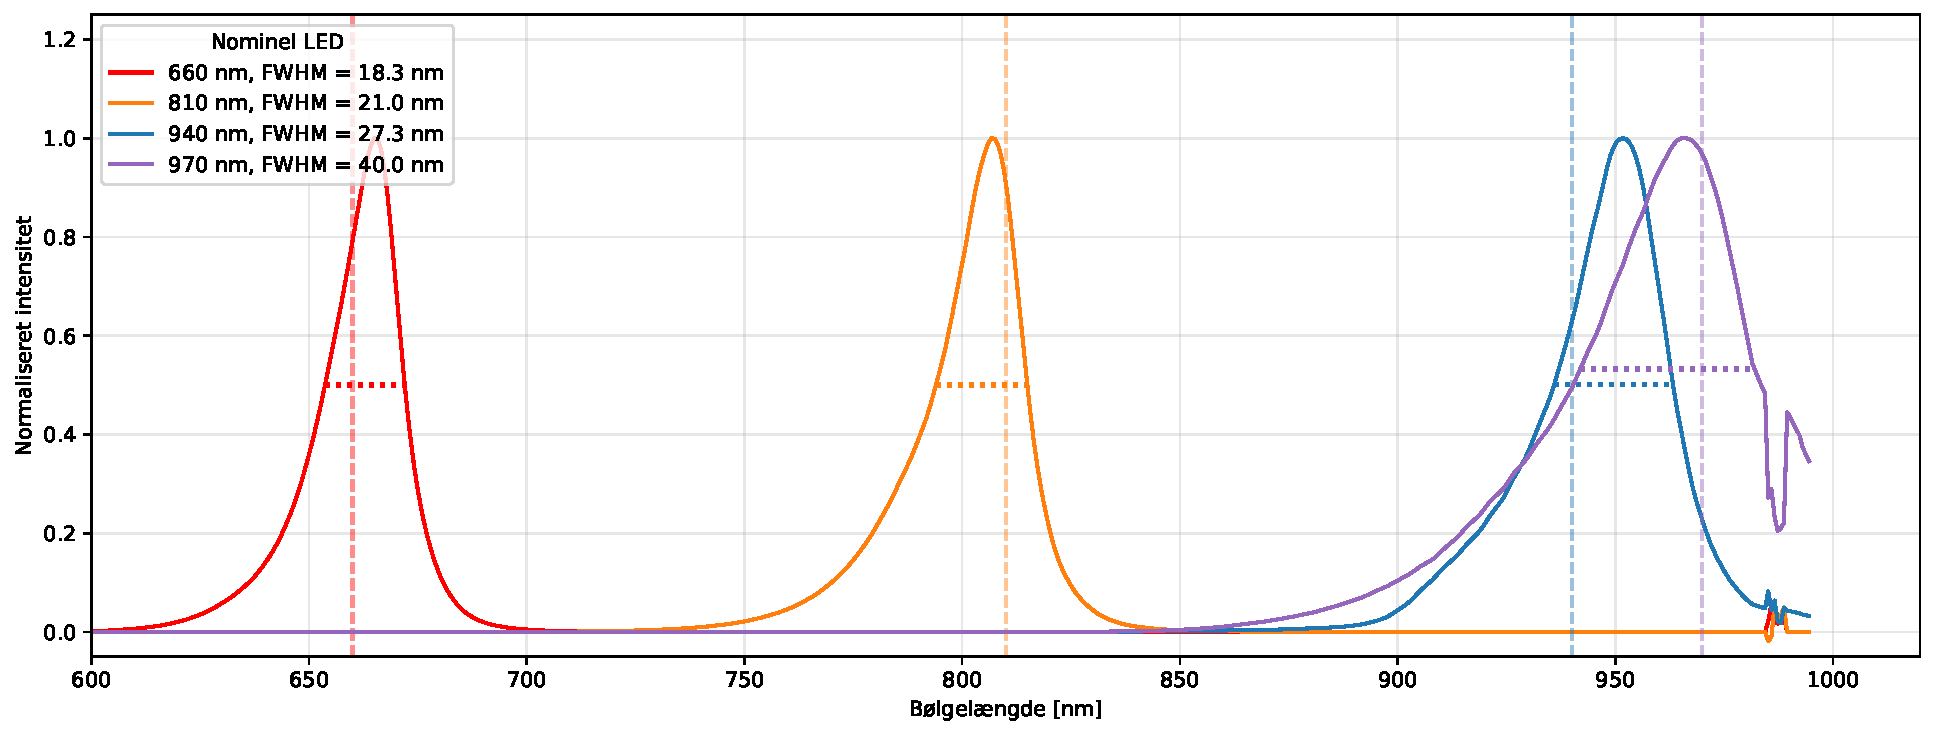
\includegraphics[width=1\linewidth]{Pictures/Graphs/led_spectra_normalized_comparison.pdf}
    \caption{Karakterisering via spektrometer af LED'er med FWHM angivet, og lodret stiplet linje ved peak intensitet i datasheet. Bemærk hotpixel/støj ved ~\SI{990}{nm}.}
    \label{fig:Karakteriserede_leder}
\end{figure}

\begin{table}[!ht]
    \centering
    \caption{LED karakteristikker} % Moved outside the tabular environment
    \label{tab:LED_karakteristikker}
    \begin{tabular}{|l|l|l|l|}
        \hline
        LED & Målt peak [nm] & Afvigelse [nm] & FWHM [nm] \\ 
        \hline
        660 nm & 664.99 & 4.99 & 18.30   \\
        \hline
        810 nm & 806.73 & -3.27 & 20.98  \\
        \hline
        940 nm & 951.79 & 11.79 & 27.25  \\
        \hline
        970 nm & 965.58 & -4.42 & 40.00  \\
        \hline
    \end{tabular}
\end{table}


\begin{figure}
    \centering
    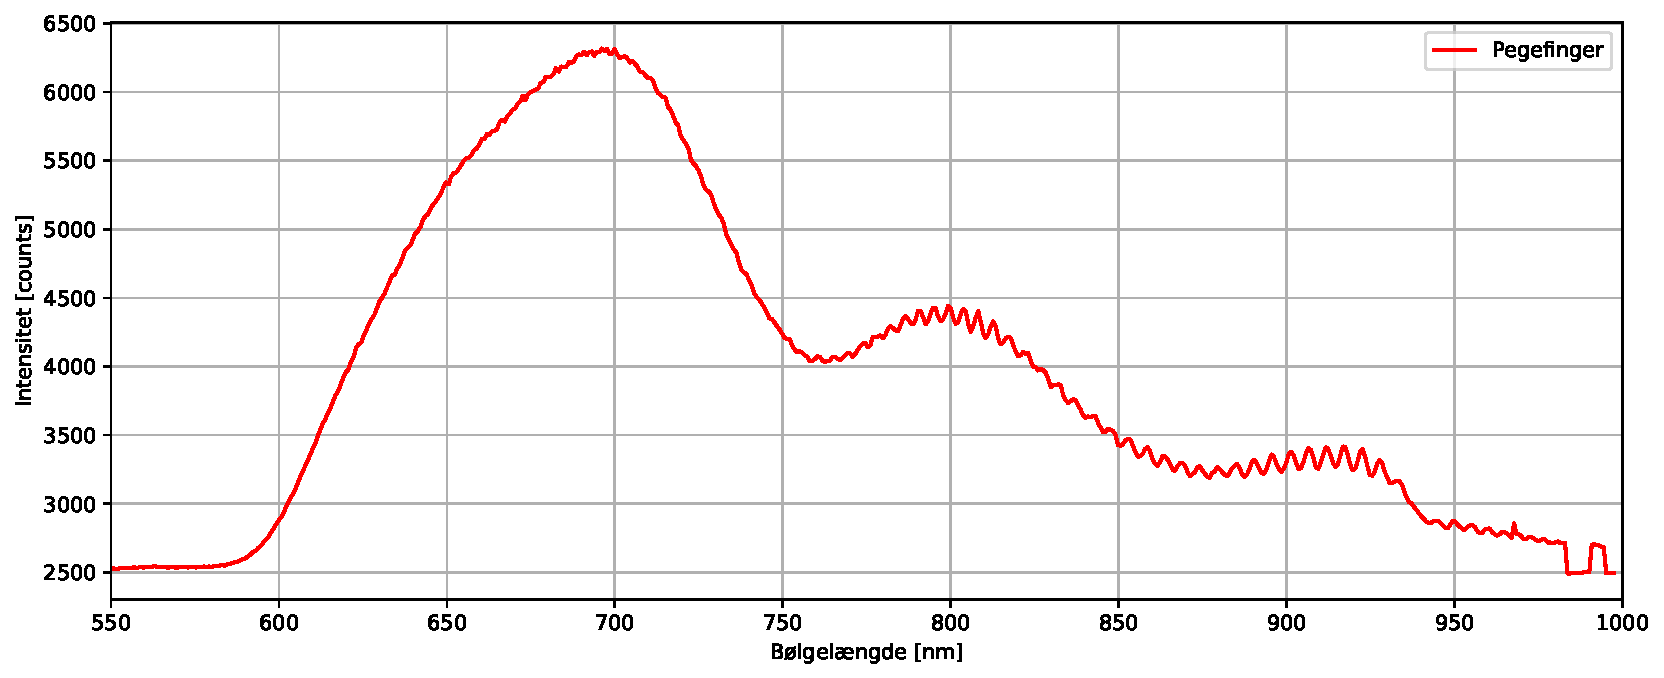
\includegraphics[width=1\linewidth]{Pictures/Graphs/Finger_spektrum.pdf}
    \caption{Karakterisering af pegefinger via belysning af halogen pære.}
    \label{fig:Karakteriseret_finger}
\end{figure}

Figur \ref{fig:Karakteriseret_finger} viser det målte transmissionsspektrum gennem en pegefinger ved belysning med en halogenpære. Det målte spektrum udviser et maksimum omkring 696 nm og aftager derefter mod længere bølgelængder, dog med lokale variationer i det nær-infrarøde område. Målingen kan ikke fortolkes som vævets absorption alene, da den også er påvirket af halogenkildens eget spektrum, spektrometerets respons og den samlede optiske geometri. Resultatet anvendes derfor primært som en kvalitativ indikation af, hvilke spektrale områder der transmitteres gennem fingeren under de givne målebetingelser

\begin{figure}
    \centering
    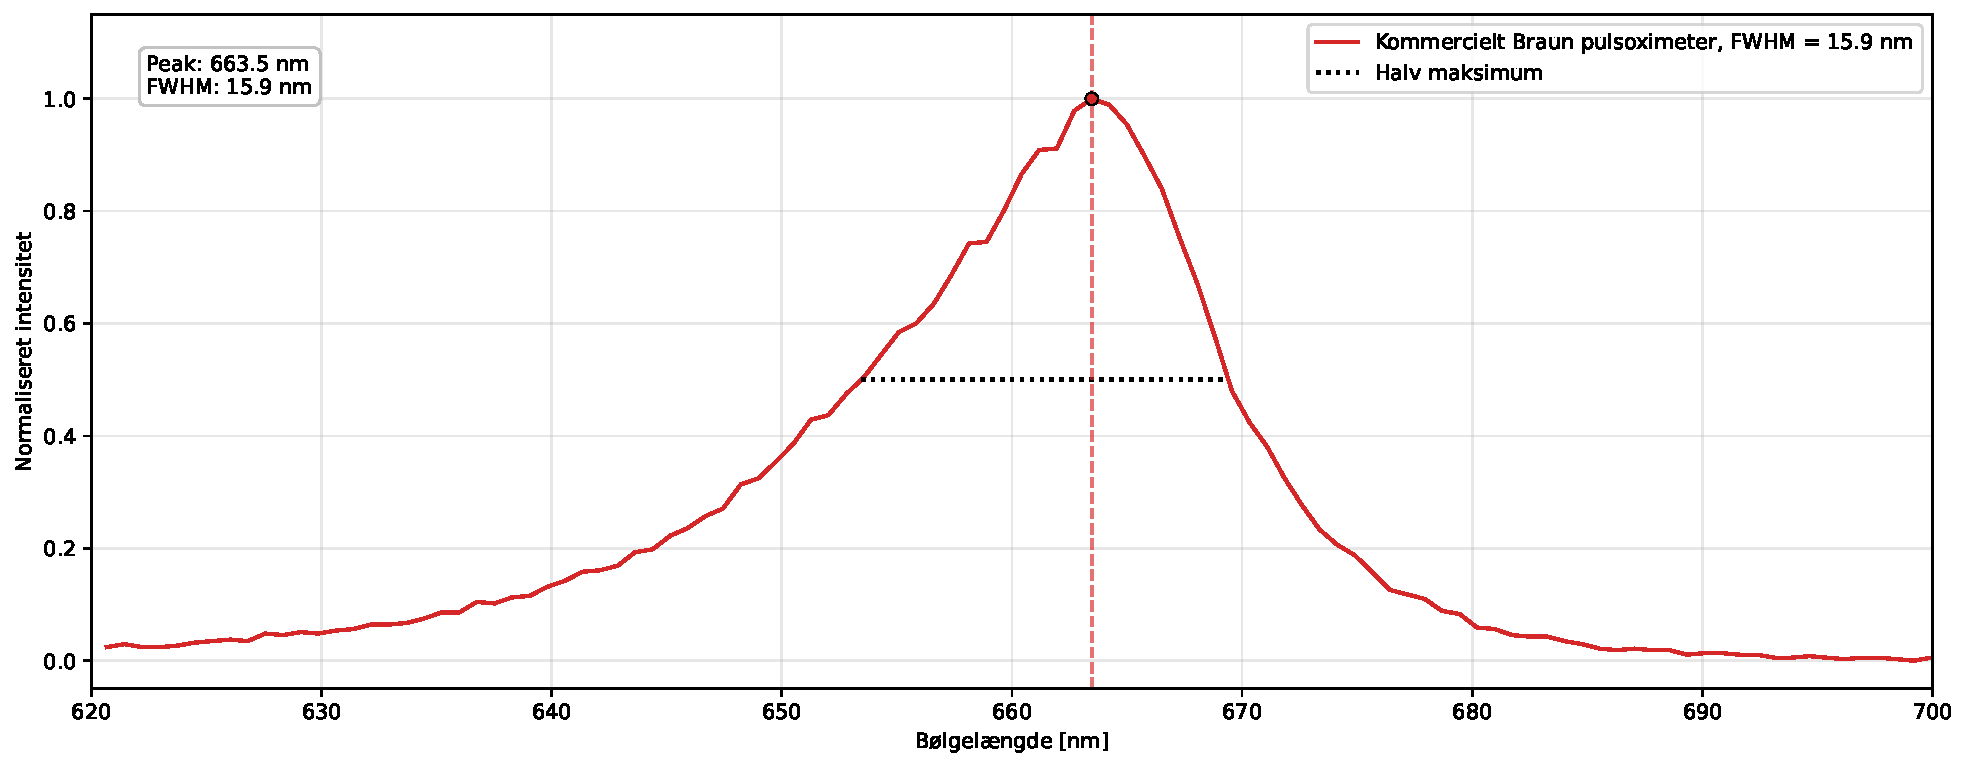
\includegraphics[width=1\linewidth]{Pictures/Graphs/Braun_pulsoximeter.pdf}
    \caption{Karakterisering af Braun puloximeter bølgelængde.}
    \label{fig:braun}
\end{figure}

Figur \ref{fig:braun} viser den spektrale karakterisering af et kommercielt Braun-pulsoximeter. Det målte emissionsmaksimum for den registrerede kanal lå ved 663.5 nm med en FWHM på 15.9 nm. Denne værdi ligger tæt på både den nominelle røde pulsoximeterkanal omkring 660 nm og den målte værdi for projektets egen røde LED. Resultatet understøtter derfor, at den valgte røde kanal i det udviklede system ligger i samme spektrale område som en kommerciel reference.

\section{Hyperspektrale resultater}
% Vis relative transmissionsresultater ved de valgte bølgelængder.
%
% Figur:
% % Eksempelbilleder ved fx 810 og 930/940 nm.
% % Plot af ROI-intensitet som funktion af bølgelængde.
%
% Vigtigt:
% % Vær forsigtig med at konkludere "størst intensitet = bedst" uden nuance.
% % Skriv "relativ transmission under de givne målebetingelser".

\begin{figure}
    \centering
    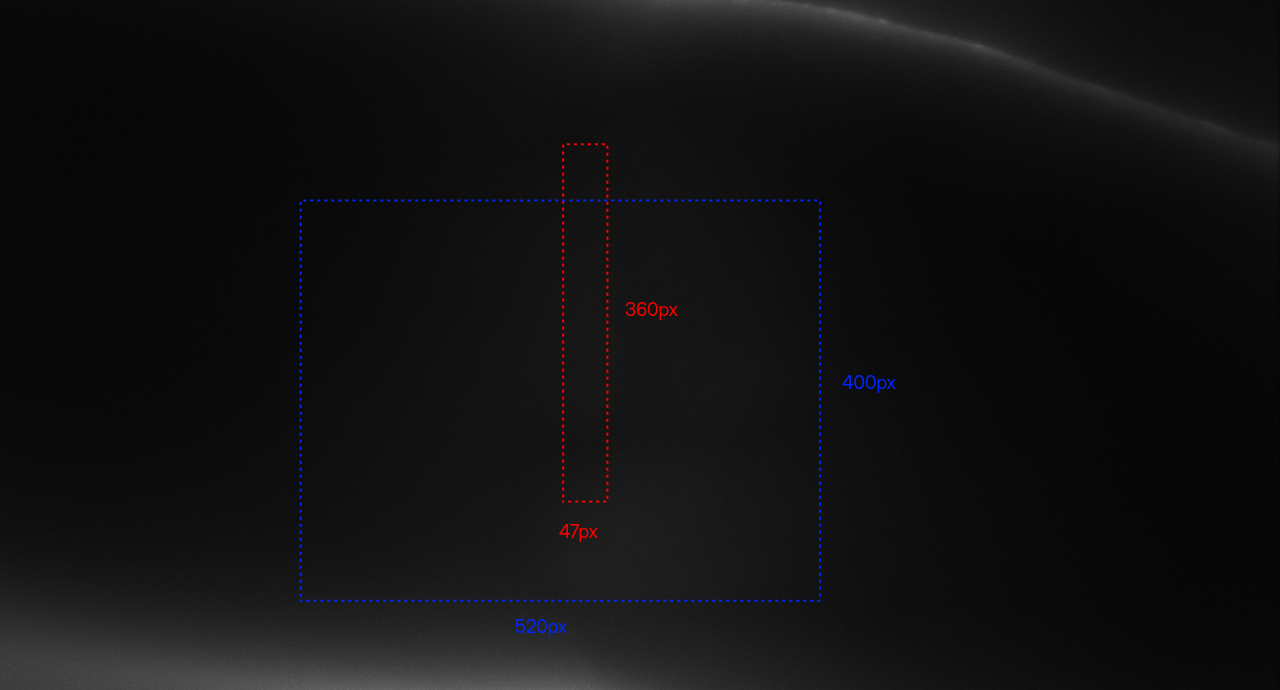
\includegraphics[width=1\linewidth]{Pictures/Other/finger_930nm_roi_regioner.png}
    \caption{Zoomet billede af fingeropsætning, med indtegnede ROI.}
    \label{fig:ROI_zoom}
\end{figure}

Figur \ref{fig:ROI_zoom} viser den anvendte billedanalyse, hvor to forskellige regioner af interesse blev udvalgt i fingerbilledet. Formålet var at undersøge, om den observerede bølgelængdeafhængighed var robust over for valg af ROI. Den store ROI dækker et bredere område af fingeren, mens den smalle centrale ROI fokuserer på den mest transmitterende del af signalet. Desuden, via det lineært variable filter mellem finger og kamera, lukkes der ikke kun en bølgelængde igennem filteret, men et smalt spænd, den fungerer derfor som et båndpas filter.

Dette spænd af bølgelængder bliver større jo større spændet er, for at modvirke dette, fungerer den smalle kolonne ROI i figur \ref{fig:ROI_zoom} som en bedre repræsentation af den valgte bølgelængde af den lineære stage, sammenlignet med den større firkantede ROI.

\begin{figure}
    \centering
    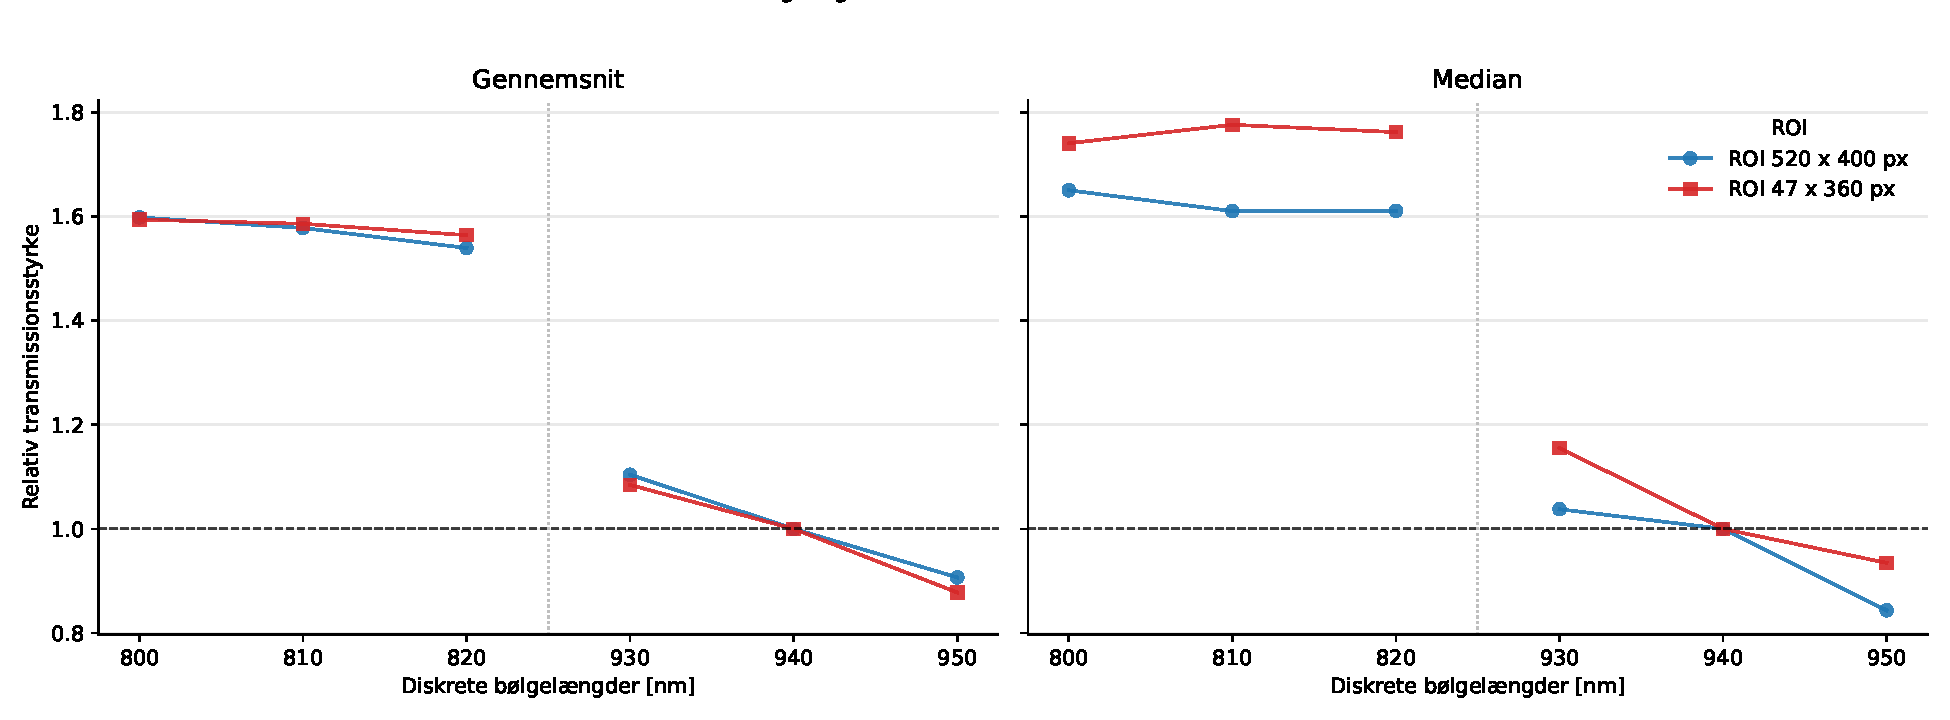
\includegraphics[width=1\linewidth]{Pictures/Graphs/Hyperspect_trans_twoROI.pdf}
    \caption{Sammenligning med gennemsnit og median af pixelintensiteter.}
    \label{fig:ROI_transmissionsværdier}
\end{figure}

Figur \ref{fig:ROI_transmissionsværdier} viser de relative transmissionsværdier beregnet ud fra både gennemsnit og median af pixelintensiteterne i de to valgte ROI’er. For begge analysemetoder ses den samme overordnede tendens, hvilket indikerer, at resultatet ikke alene skyldes det præcise valg af ROI. Samtidig ses mindre forskelle i de absolutte værdier mellem gennemsnits- og medianbaseret analyse, særligt for den smalle ROI, hvilket viser, at den numeriske værdi er følsom over for den valgte statistik. Den overordnede rangordning mellem bølgelængderne bevares dog, og resultatet peger derfor på, at de observerede forskelle er reelle under de givne målebetingelser.


\section{Elektroniske delresultater}
% Dokumentér at delkredsløb virker.
% Hold det kort og fokuseret.
%
% Figur:
% % Et eller to nøgleplots af signal gennem kæden eller karakterisering af gain/støj.
Figur \ref{fig:TIA_output} viser outputtet fra TIA-stadiet før yderligere analog filtrering. Det rå signal består af tre gentagne faser svarende til de to LED-målinger samt mørkemålingen. Derudover ses en tydelig 50 Hz-komponent med en amplitude omkring \SI{160}{mV}, hvilket viser, at signalet på dette stadie stadig er påvirket af netstøj og omgivelsesrelaterede interferenskilder.
\begin{figure}[htbp]
    \centering
    \includegraphics[width=1\textwidth]{Pictures/Graphs/TIA_output.png}
    \caption{Udsnit af oscilloskop output efter TIA.}
    \label{fig:TIA_output}
\end{figure}

Efter lavpasfiltrering, vist i figur \ref{fig:LPF_output}, reduceres de hurtigste variationer og \SI{50}{Hz} støj i signalet. Multiplexstrukturen kan stadig observeres, men signalet fremstår væsentligt glattere end direkte efter TIA-stadiet. Dette viser, at lavpasfilteret bidrager til at begrænse højfrekvent støj uden at fjerne den overordnede signalstruktur.

\begin{figure}[htbp]
    \centering
    \includegraphics[width=1\textwidth]{Pictures/Graphs/LPF_output.pdf}
    \caption{LPF output ved 4.17 Hz multipleksing.}
    \label{fig:LPF_output}
\end{figure}

Figur \ref{fig:gain_output} viser signalet efter det afsluttende gain-stadie. Her ses, at signalamplituden er hævet til et niveau, der udnytter dataopsamlingens dynamiske område bedre. Samtidig bevares den tidslige struktur fra de foregående stadier, hvilket indikerer, at forstærkningen ikke har introduceret væsentlig forvrængning af signalformen.

\begin{figure}[htbp]
    \centering
    \includegraphics[width=1\textwidth]{Pictures/Graphs/gain_output.pdf}
    \caption{Udsnit af oscilloskop output efter gain stadiet}
    \label{fig:gain_output}
\end{figure}

\section{PPG-resultater fra det analoge system}
% Dette er hovedsektionen i resultatkapitlet.
%
% Figur:
% % Råt tidsdomænesignal
% % Filtreret PPG
% % Rød og IR sammenlignet
% % Zoom på 2--3 pulscykler
%
% Tabel:
% % Målt pulsrate
% % AC/DC eller signalamplitude
% % evt. R-værdier

Figur \ref{fig:pulsox_final} viser en live-måling med det endelige pulsoximetersystem ved 7.17 Hz multiplexing. De to optiske kanaler ved 660 nm og 940 nm kan følges over tid, og på baggrund af disse signaler blev både puls og SpO$_2$ estimeret i realtid. I det viste eksempel blev der for den valgte analyseperiode opnået en middelværdi for pulsen på $51.7 \ \pm \ 0.3$ BPM og et middelestimat for SpO$_2$ på $95.8 \ \pm \ 1.5 \%$. 

Resultatet demonstrerer, at systemet ikke blot kan registrere et optisk signal gennem fingeren, men også udtrække pulsoximetrisk relevante parametre ved efterfølgende signalbehandling. Estimatet skal dog fortolkes som et proof-of-concept, da systemet ikke er klinisk kalibreret mod arterielle blodgasmålinger(SaO$_2$).

\begin{figure}[htbp]
    \centering
    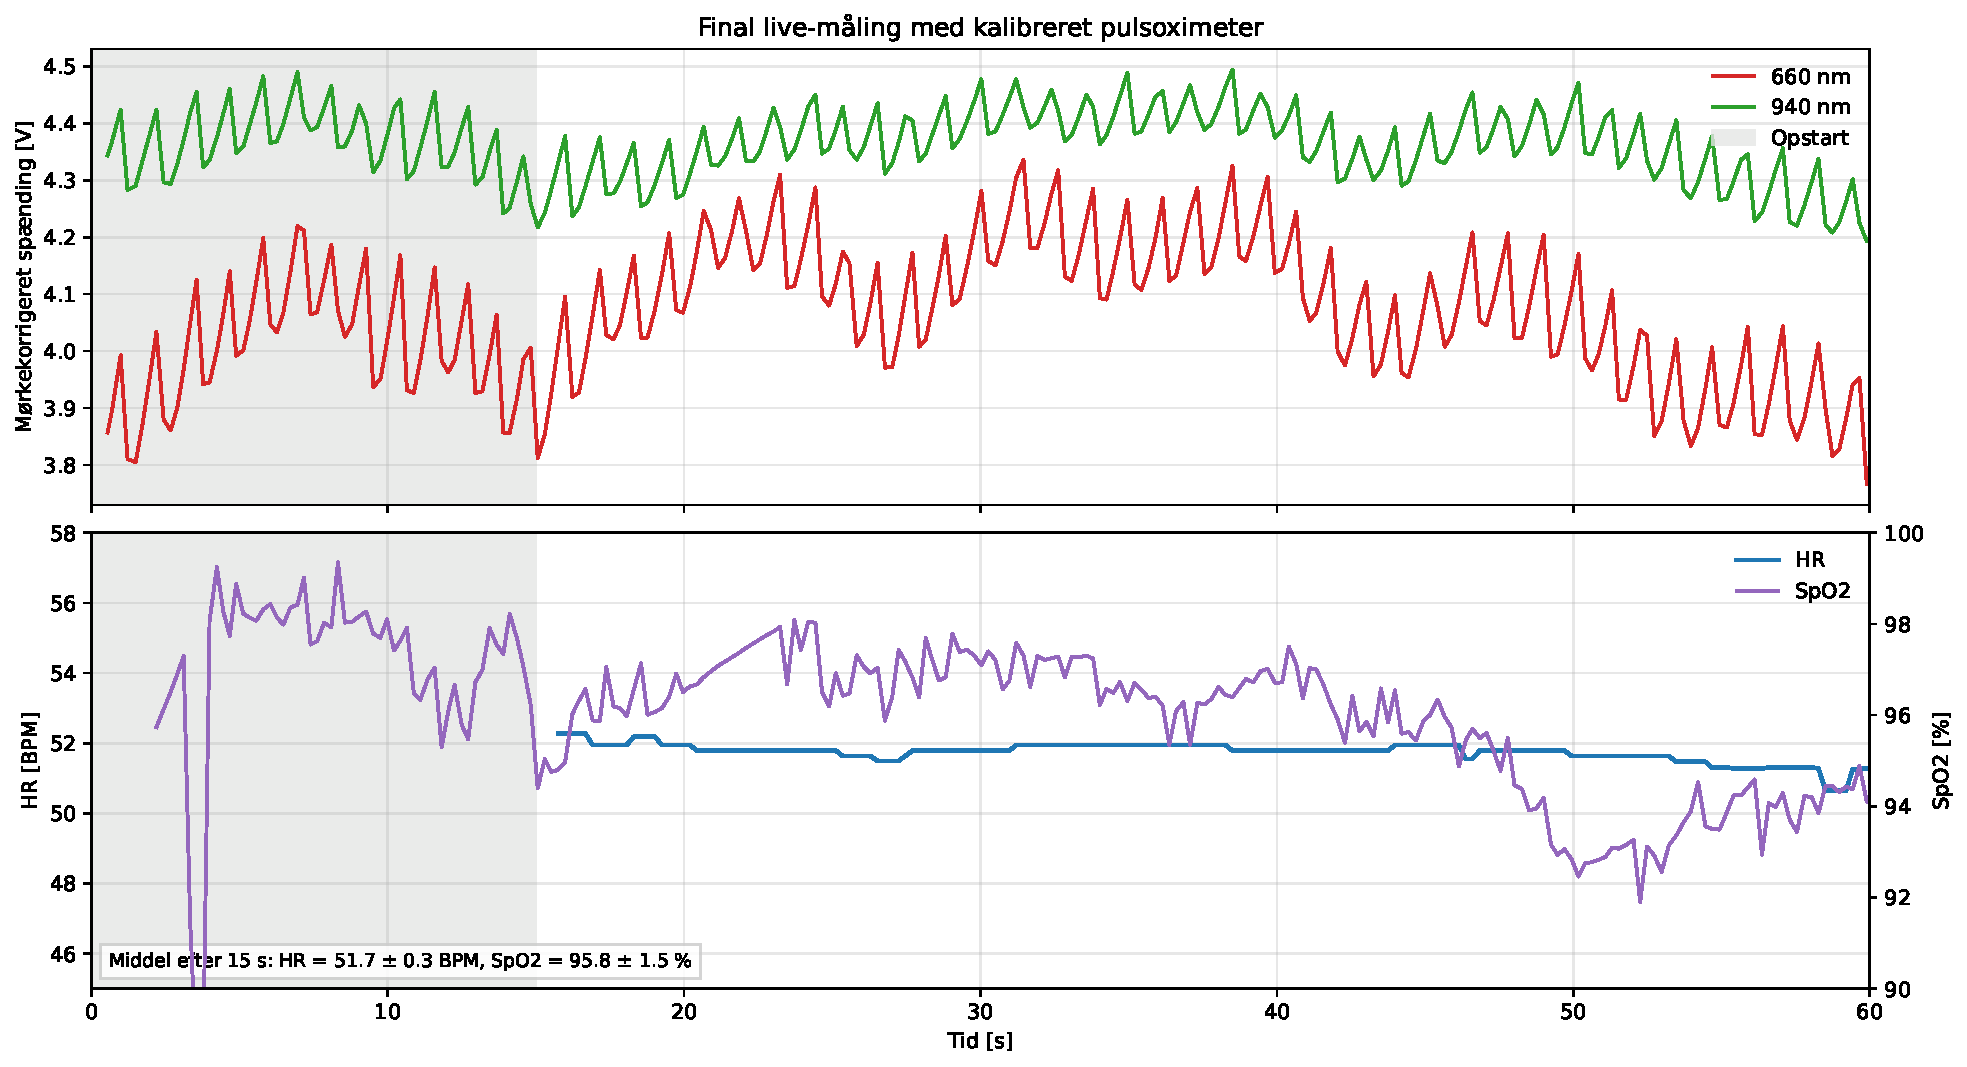
\includegraphics[width=1\textwidth]{Pictures/Graphs/live_pulsoximeter_final_demo.pdf}
    \caption{Live pulsoximeter test kørt ved \SI{7.17}{Hz}}
    \label{fig:pulsox_final}
\end{figure}


\section{Opsummering af centrale fund}
% Kort resultatsammenfatning.
% Ingen stor fortolkning endnu.

Samlet set viste resultaterne, at de valgte LED’er opererede i de ønskede spektralområder, men med målbare forskelle mellem nominelle og faktiske peak-bølgelængder. De hyperspektrale målinger viste, at de relative transmissionsværdier afhænger af både bølgelængde og valg af analysemetode, men at den overordnede tendens var robust over for ROI-valg. De elektroniske delmålinger viste desuden, at den analoge signalkæde kunne omsætte den svage fotostrøm til et brugbart spændingssignal, som efter filtrering og forstærkning muliggjorde realtidsestimering af både puls og